\section{Performance}

The response of the LTCC to electrons and pions has been studied using experimental data from the spring 2019 period,
the first time that the LTCC sectors 3 and 5 were filled with the C$_4$F$_{10}$ gas.
At the time of this writing the data is not yet fully calibrated.

\subsection{LTCC Response to Electrons}\label{sec:elecResponse}

The electrons are selected using the reconstruction algorithms~\cite{recon-nim} that identifies electron tracks.
The LTCC response is calculated by checking whether the electrons produced a signal in the detector or not.
The electron momenta has been selected in the expected pion response range, between 3.5 and 8~GeV.
The criteria for event selections are:

\begin{itemize}
   \item  Electrons identified using the reconstruction event builder algorithm;
    \item Electrons must be within the fiducial volume of the LTCC , see \F{electronDetFiducialCut}.
\end{itemize}

\begin{figure}
	\centering
	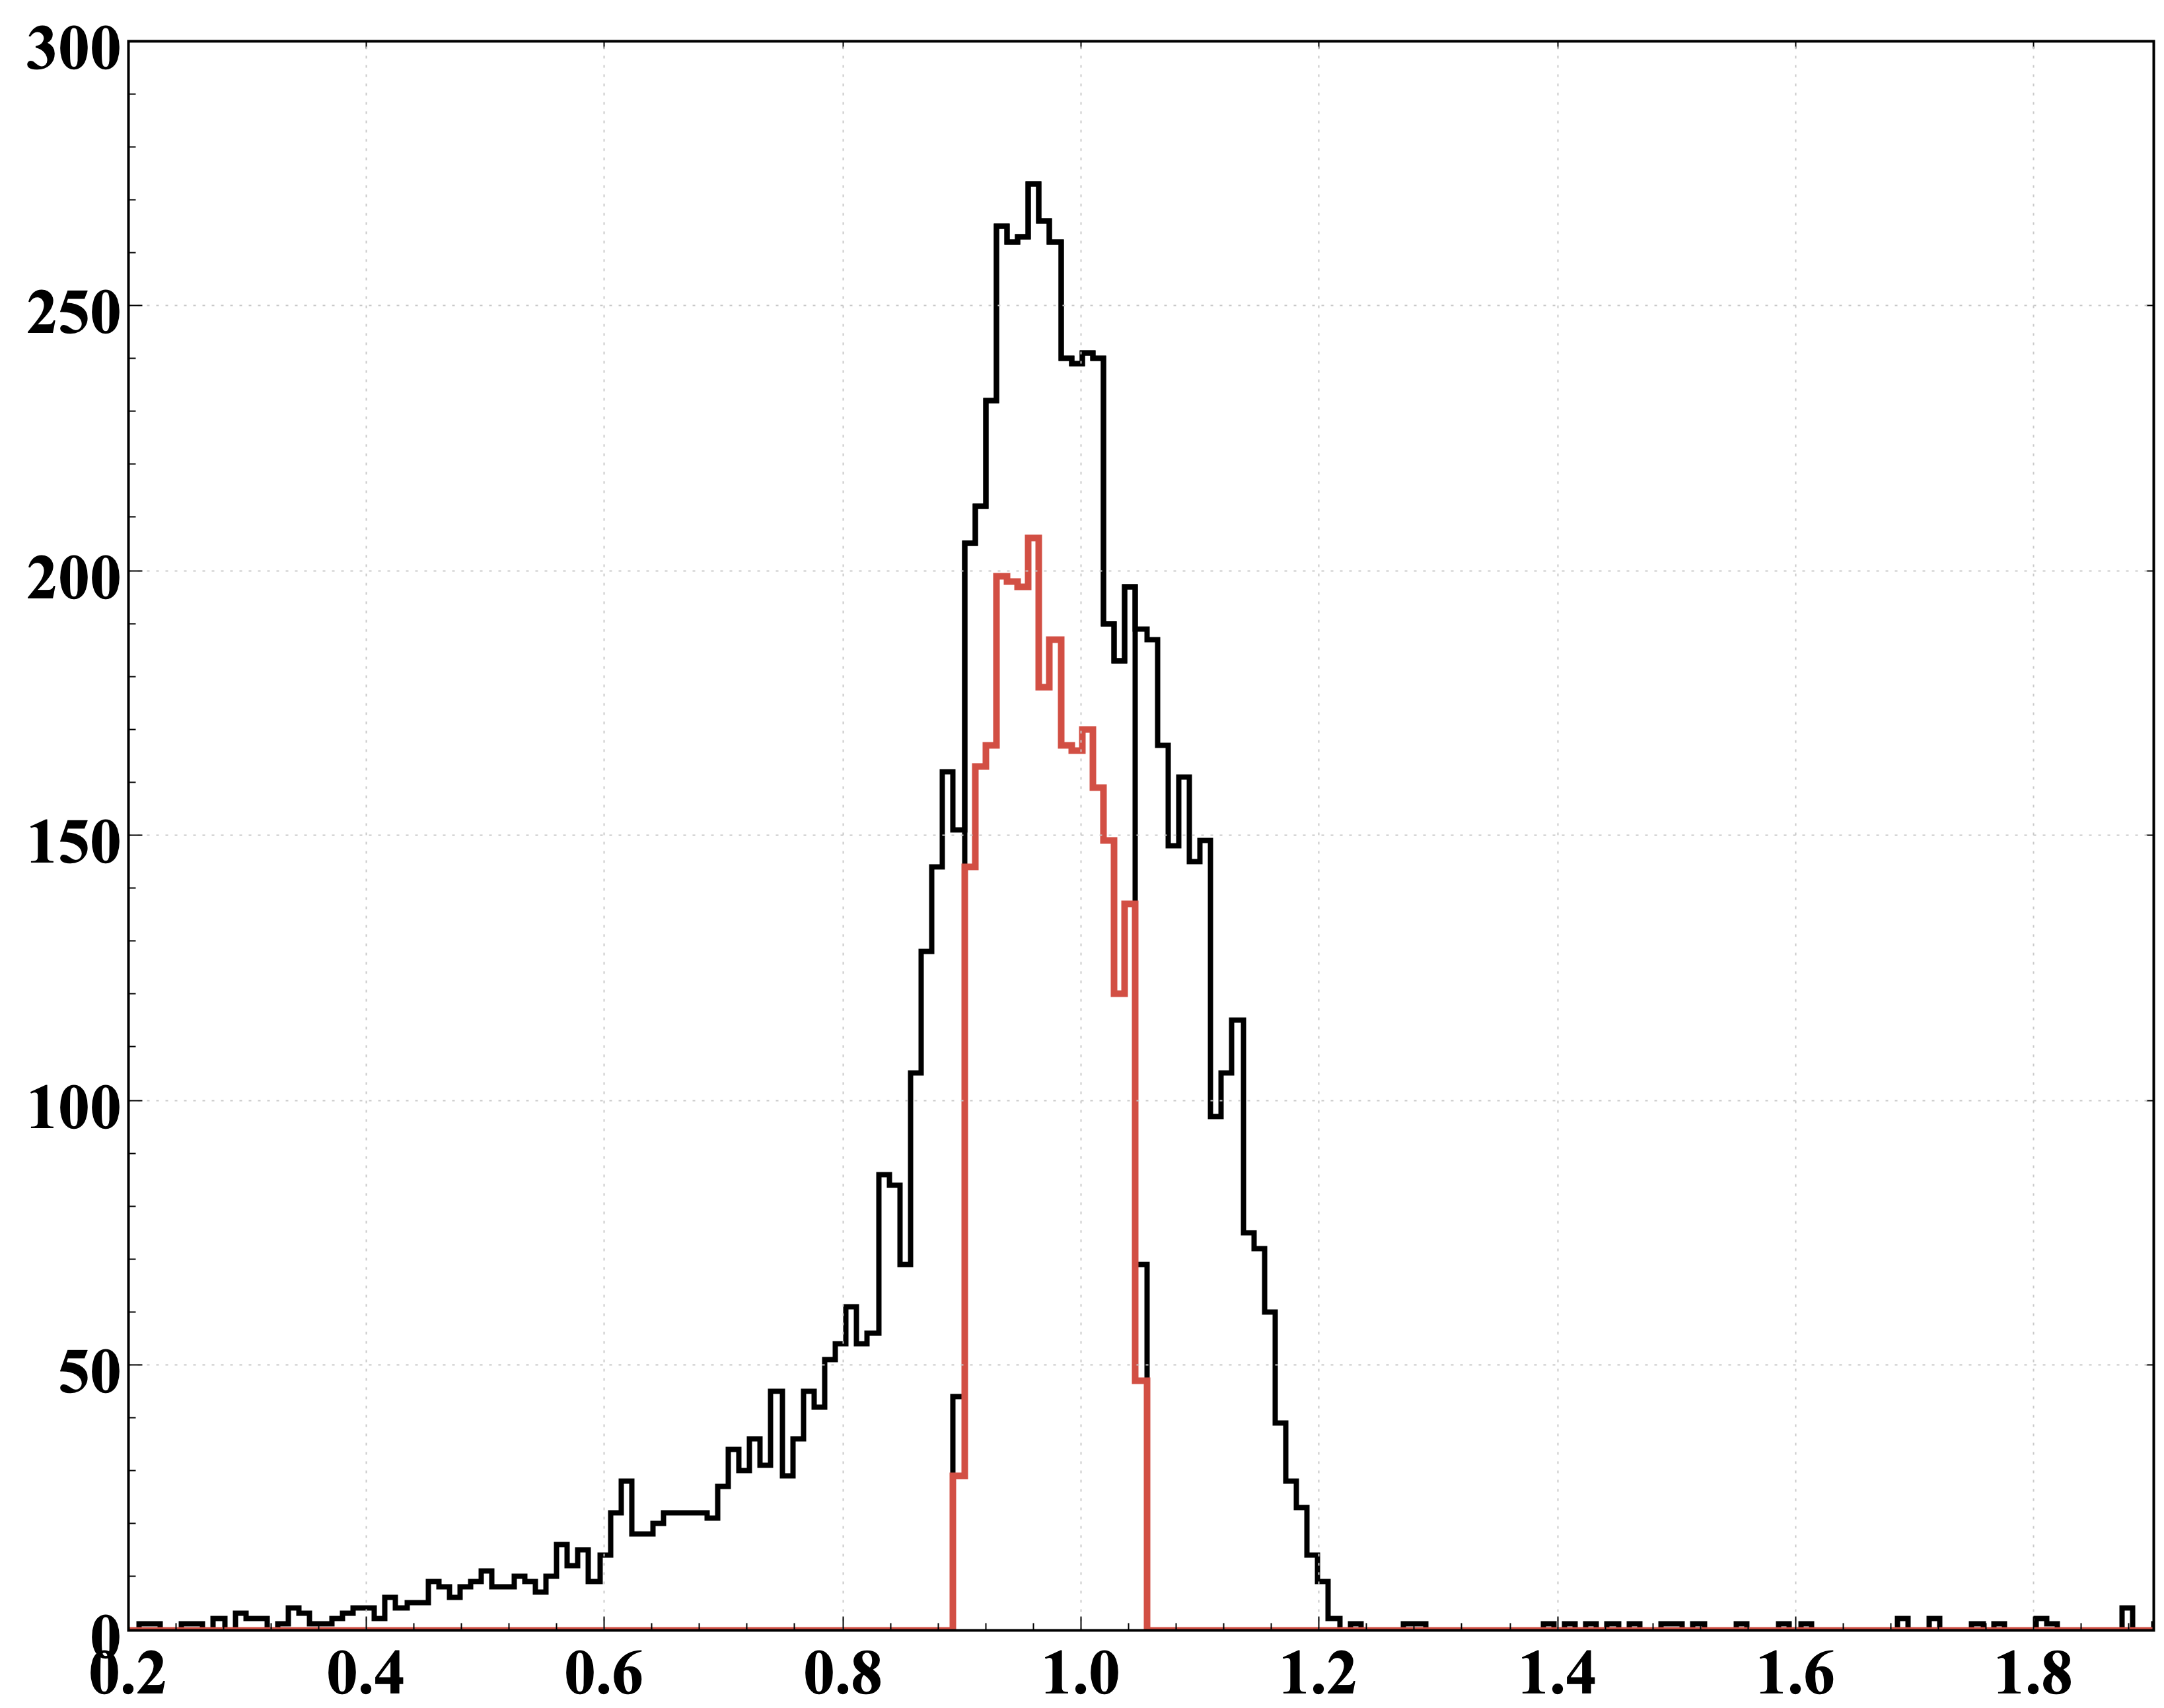
\includegraphics[width=0.98\columnwidth,keepaspectratio]{img/electronDetFiducialCut.png}
	\caption{(placeholder) The electron fiducial cut applied to electrons}
	\label{fig:electronDetFiducialCut}
\end{figure}

The electron momentum spectrum before and after the requirement of an associated LTCC signal is shown
in \F{electronEfficiency}, along with a 0$^{th}$-order polynomial fit. The average efficiency of electrons is
94$\%$, below the expected efficiency of 99$\%$. This may be due to the fact that the electron selection
did not involve the calorimeters (due to the uncalibrated detector status) and/or by unrelated inefficiencies
in other detector systems.

\begin{figure}
	\centering
	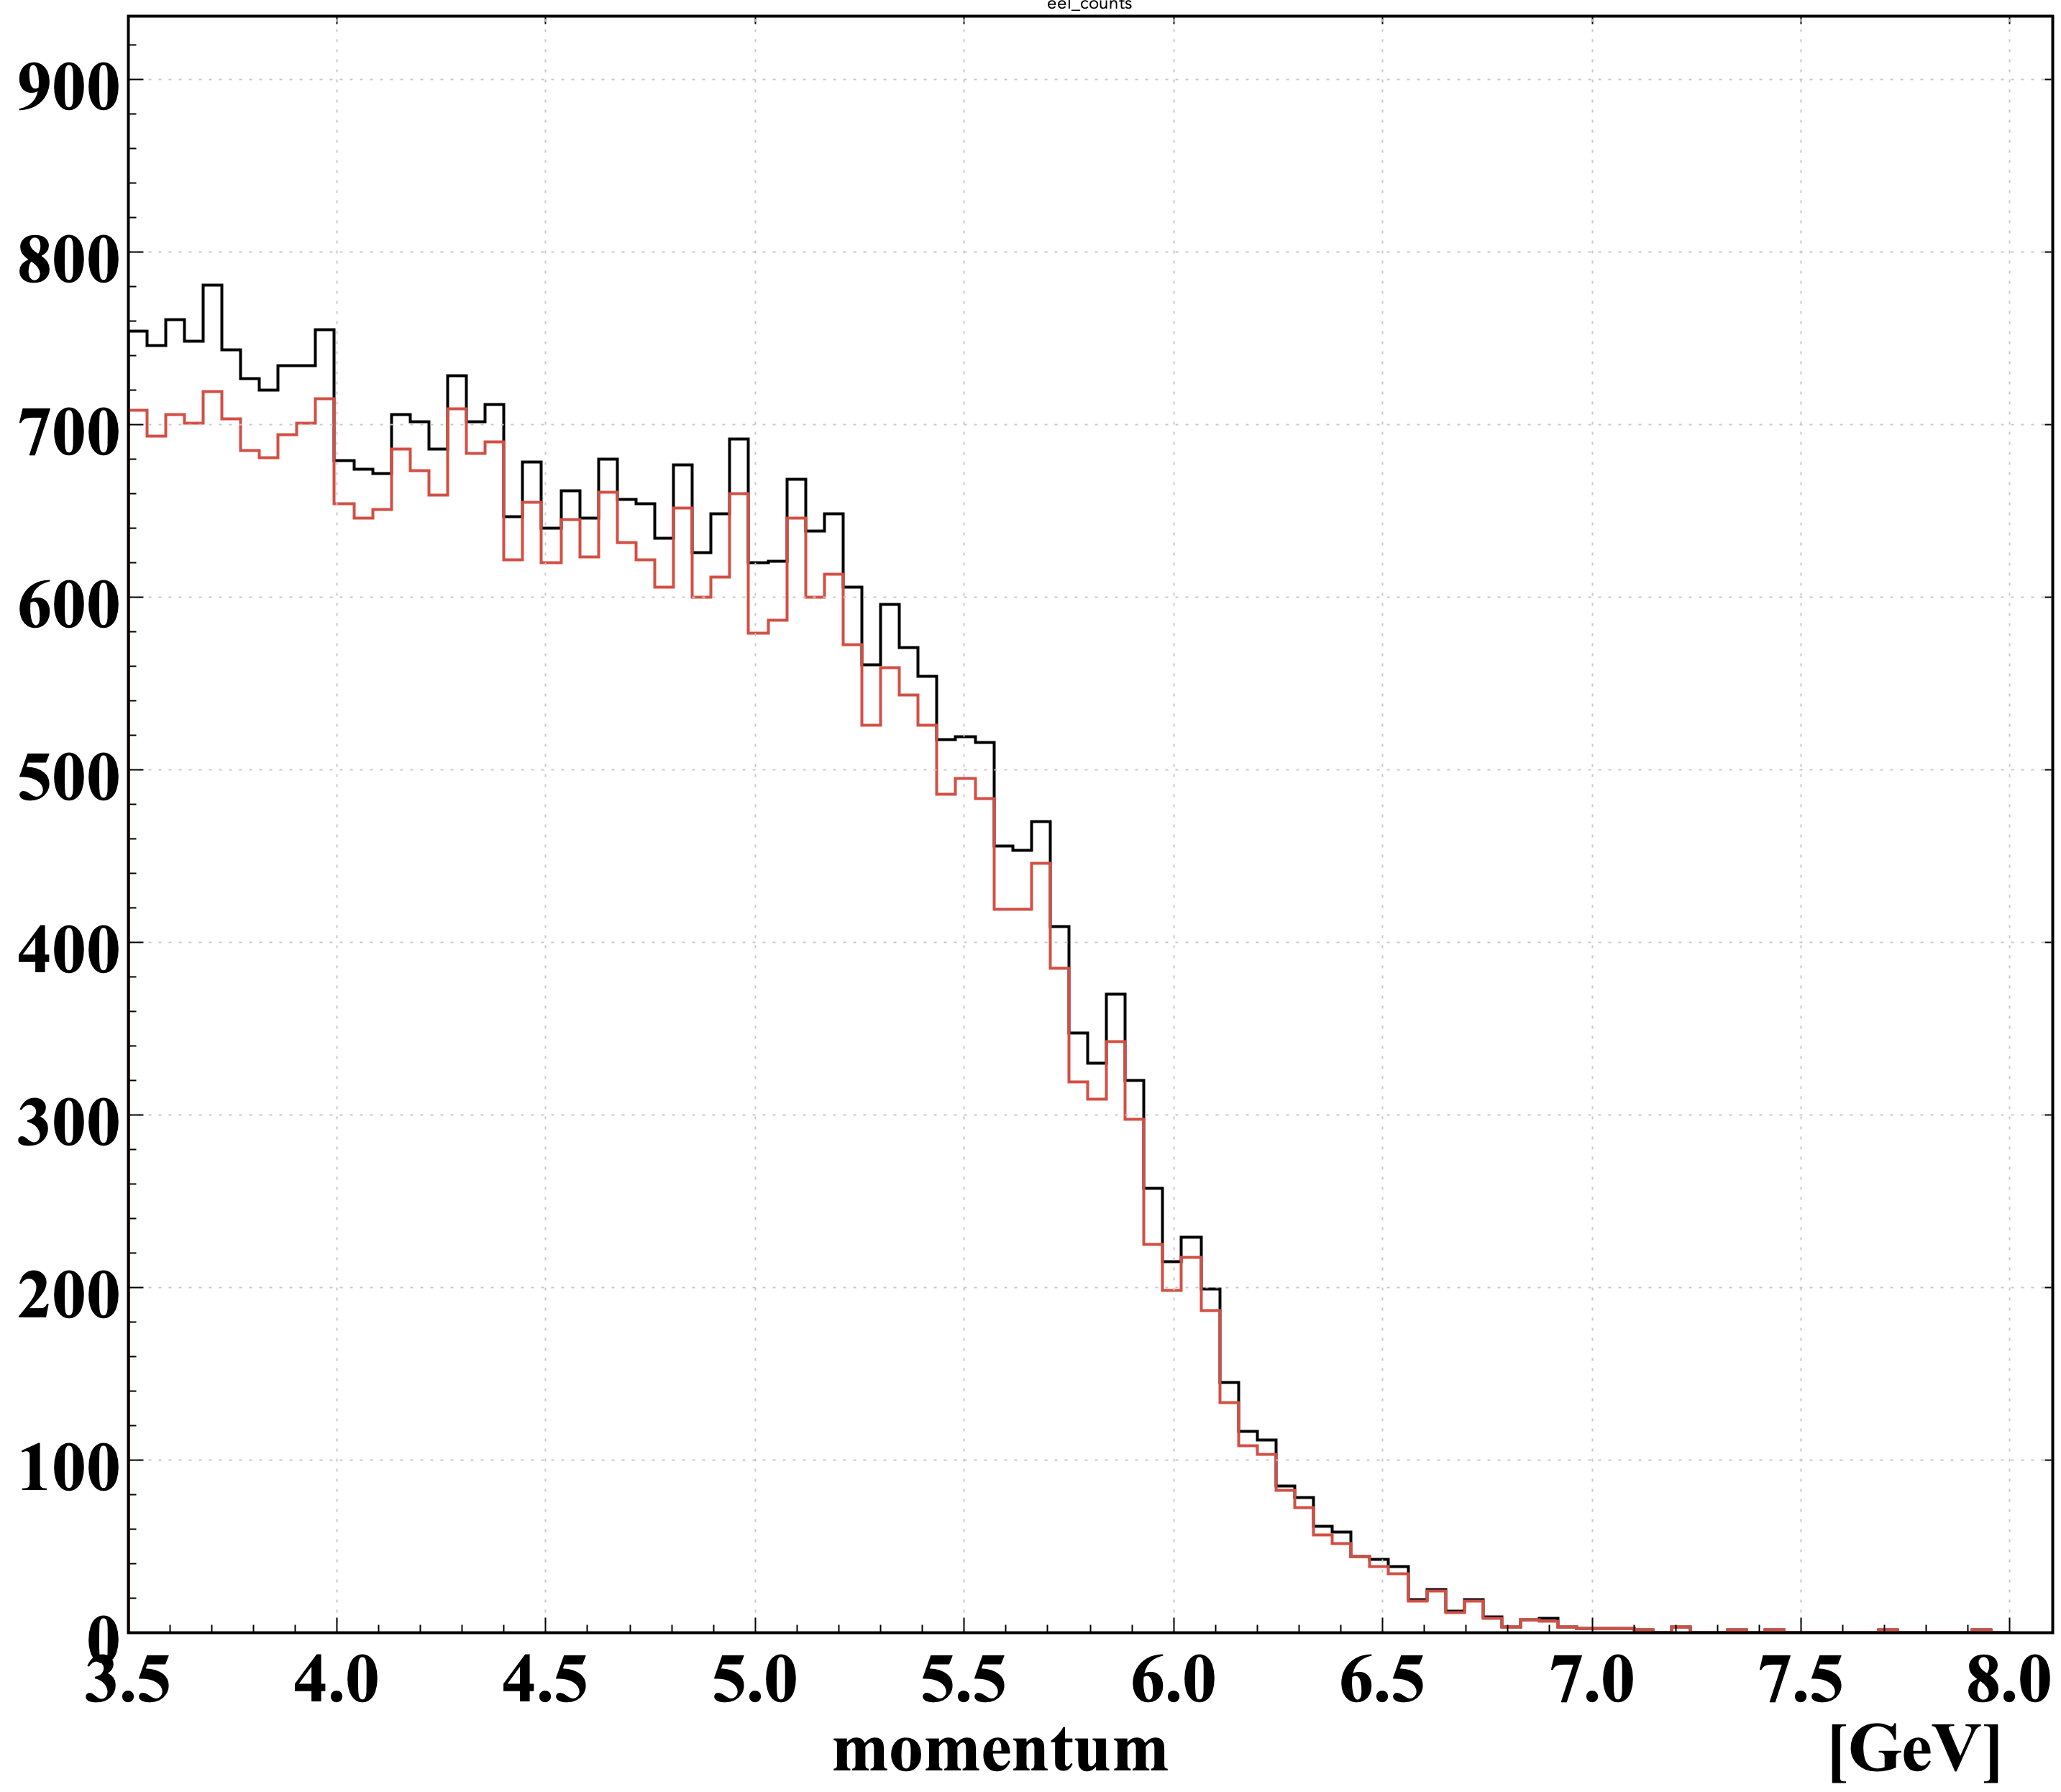
\includegraphics[width=0.98\columnwidth,keepaspectratio]{img/electronMomenta.png}
	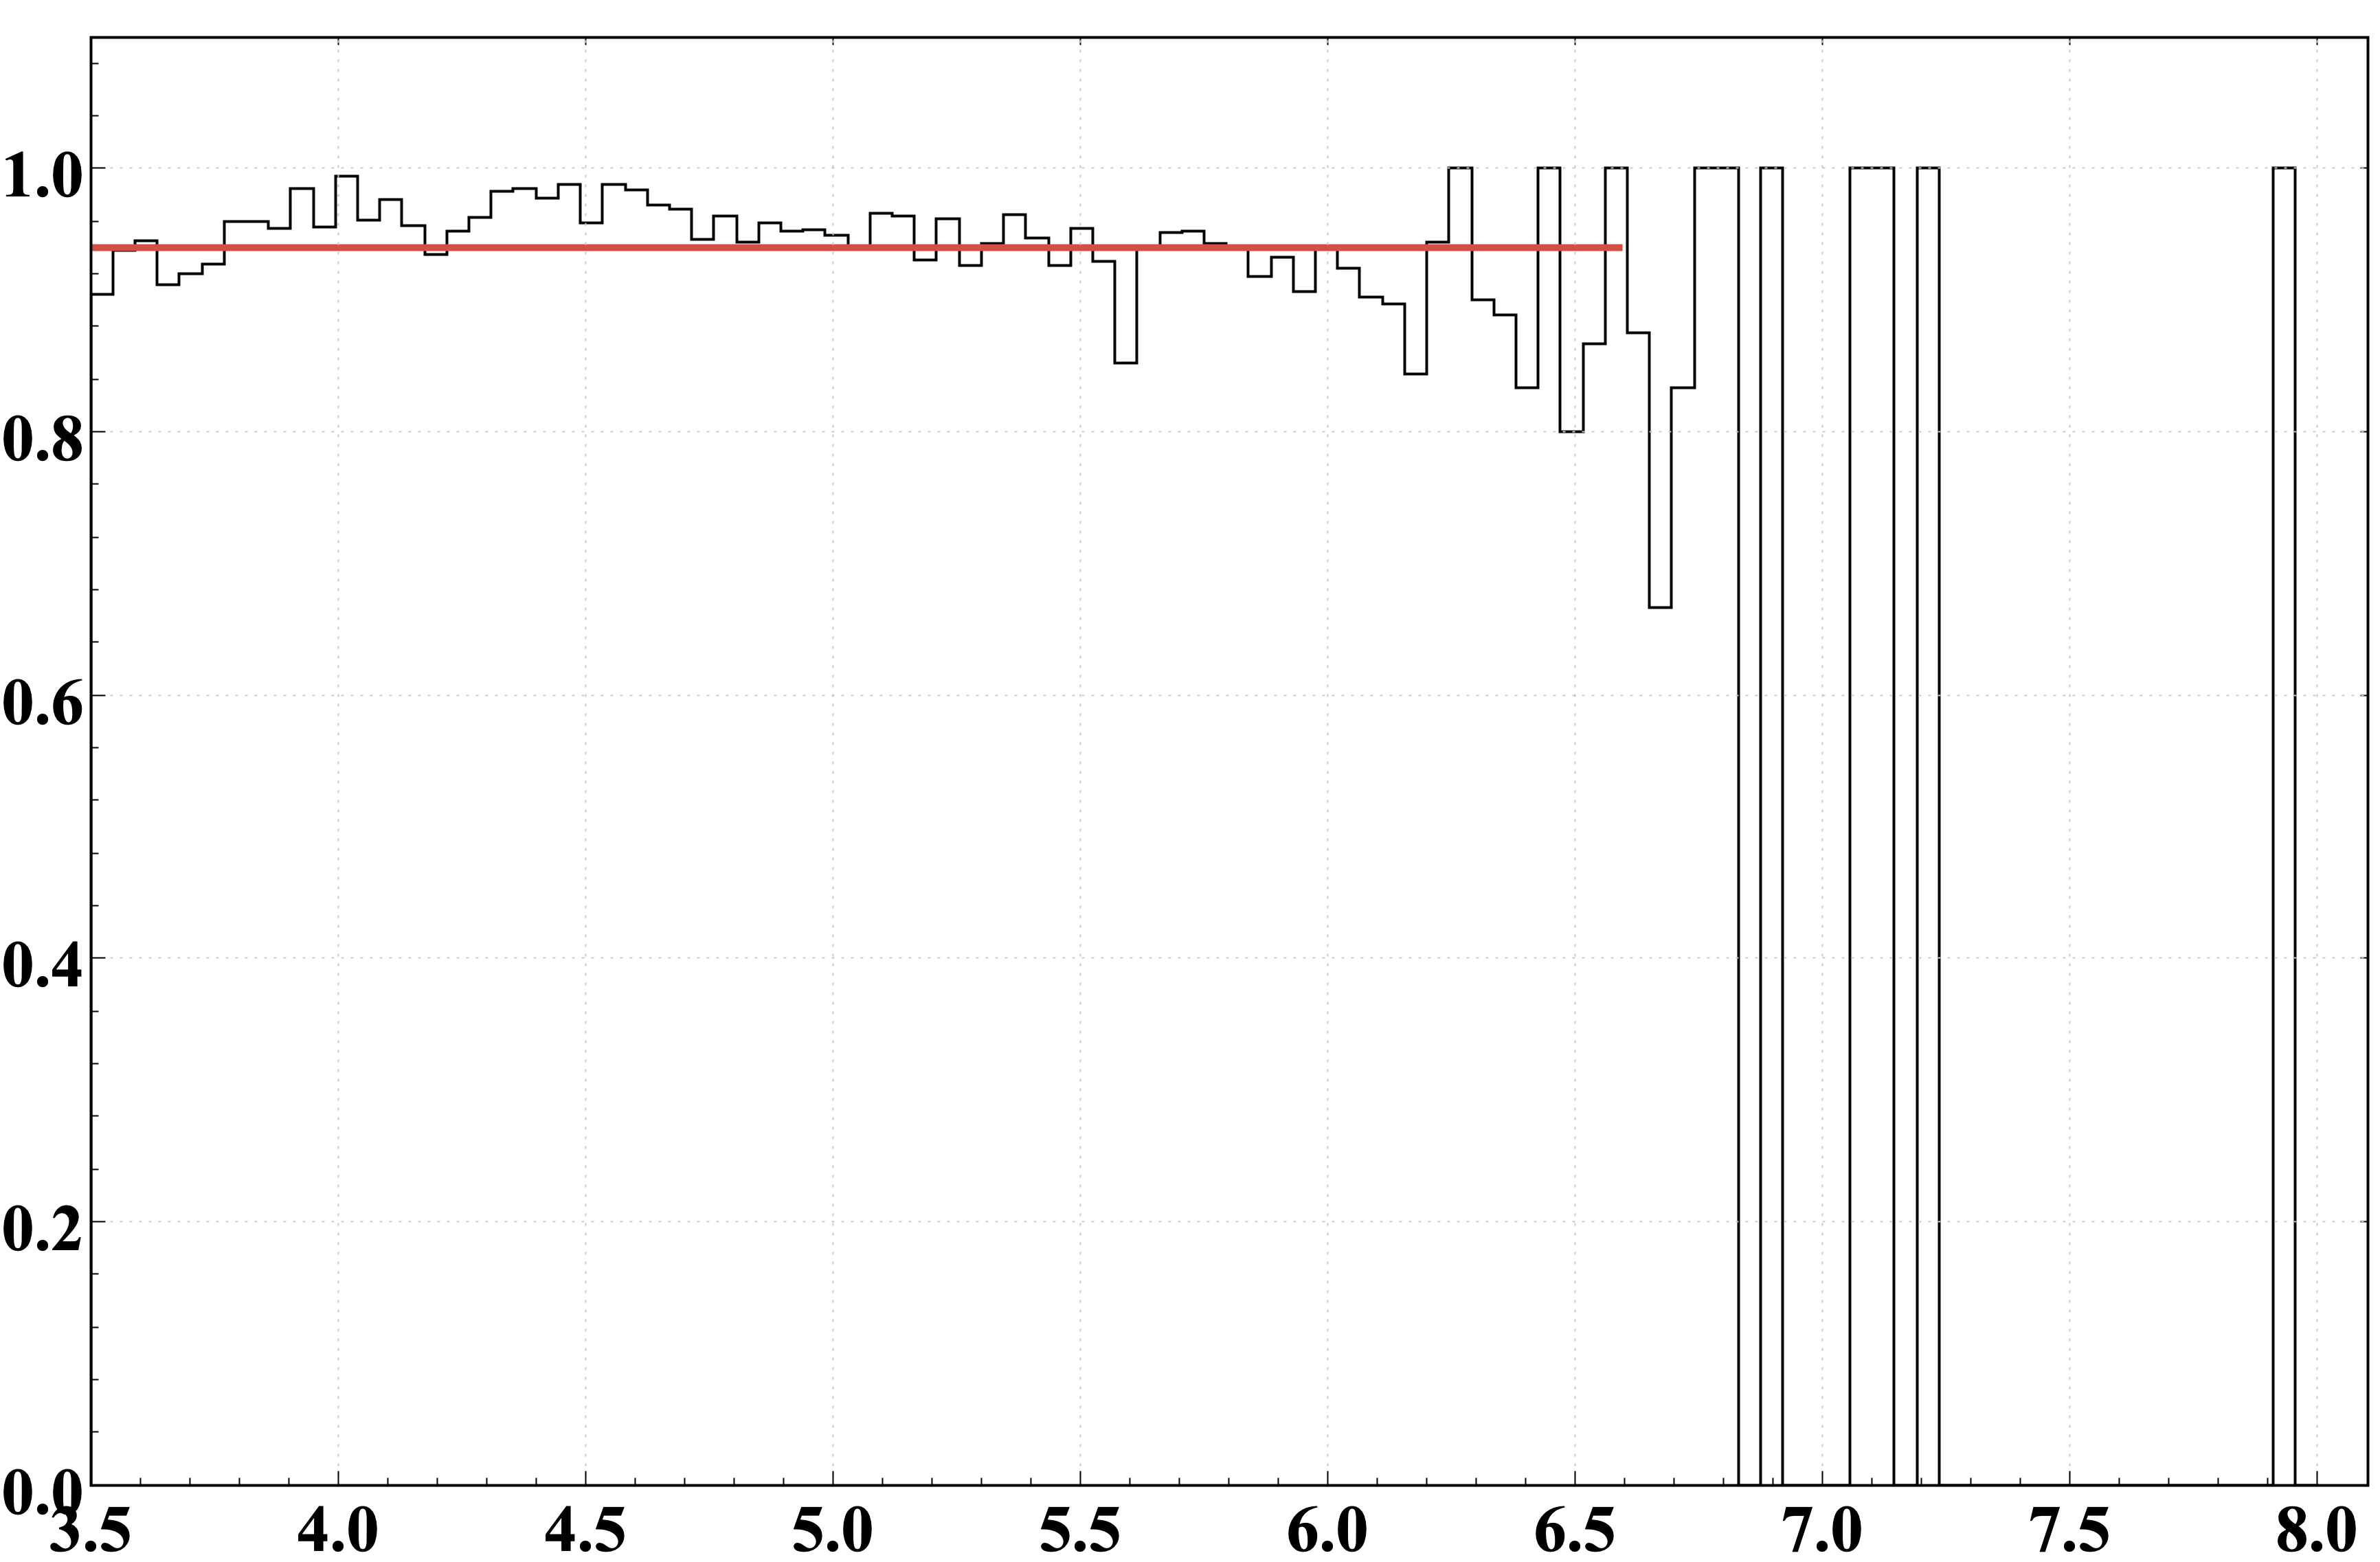
\includegraphics[width=0.98\columnwidth,keepaspectratio]{img/electronEfficiency.png}
	\caption{(placeholder) Top: the number of reconstructed electrons vs. momentum (GeV) before and
          after the requirement of an associated LTCC signal. Bottom: the LTCC efficiency to electrons is the
          ratio of the two distributions above. A 0$^{th}$-order polynomial fit gives an average of 94$\%$
          efficiency.}
	\label{fig:electronEfficiency}
\end{figure}

\subsection{LTCC Response to Pions}

The calculate the response of the LTCC to pions, reconstructed positively charged pion are selected
and a check is done on whether they produced a signal in the LTCC detector. The positive pion selection
considers all positively charged particles that pass a neutron missing mass cut for the reaction
$ep \to e'\pi^+n$. The criteria for event selection are:

\begin{itemize}
    \item The electron selection described in Section~\ref{sec:elecResponse};
    \item Positive pion candidates are identified using the reconstruction event builder algorithm;
    \item The positive pion candidates must be within the detector fiducial volume, see \F{detFiducialCut}.
    \item A neutron missing mass cut is applied between 0.9 and 1.05~GeV (see \F{neutronMM}).
\end{itemize}

\begin{figure}
	\centering
	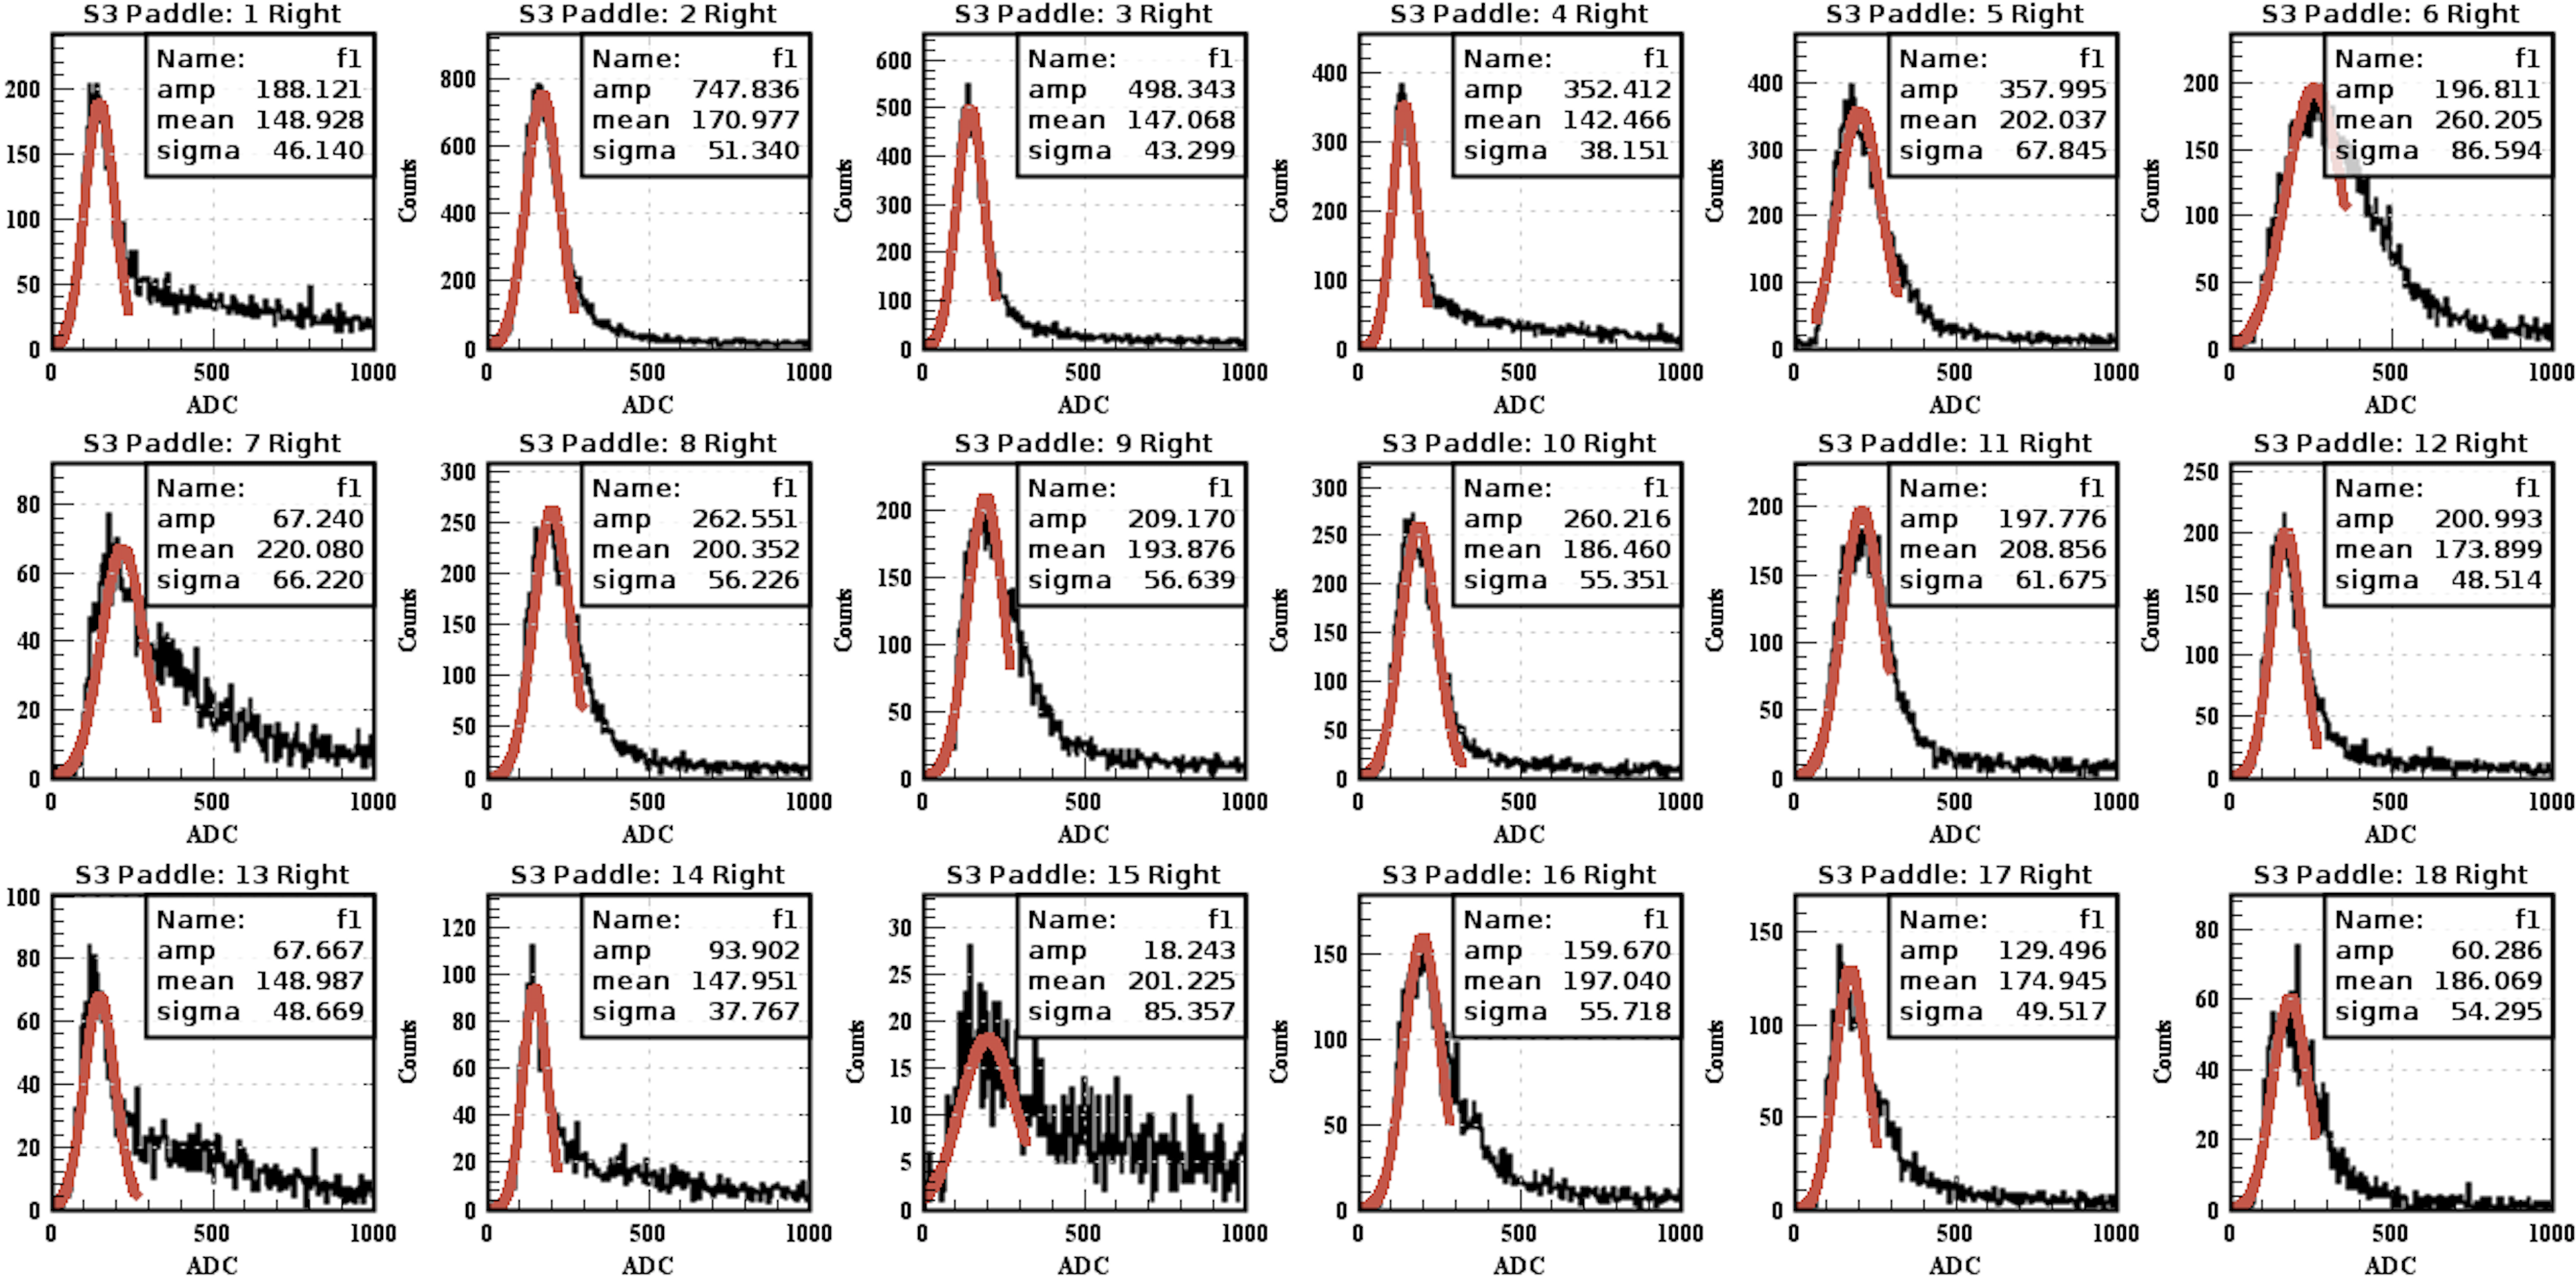
\includegraphics[width=0.98\columnwidth,keepaspectratio]{img/neutronMM.png}
	\caption{(placeholder) The fiducial cut applied to pions}
	\label{fig:detFiducialCut}
\end{figure}

The missing mass cut is shown in \F{neutronMM}. The positive pion candidates that satisfy the cuts are shown
in black.

\begin{figure}
	\centering
	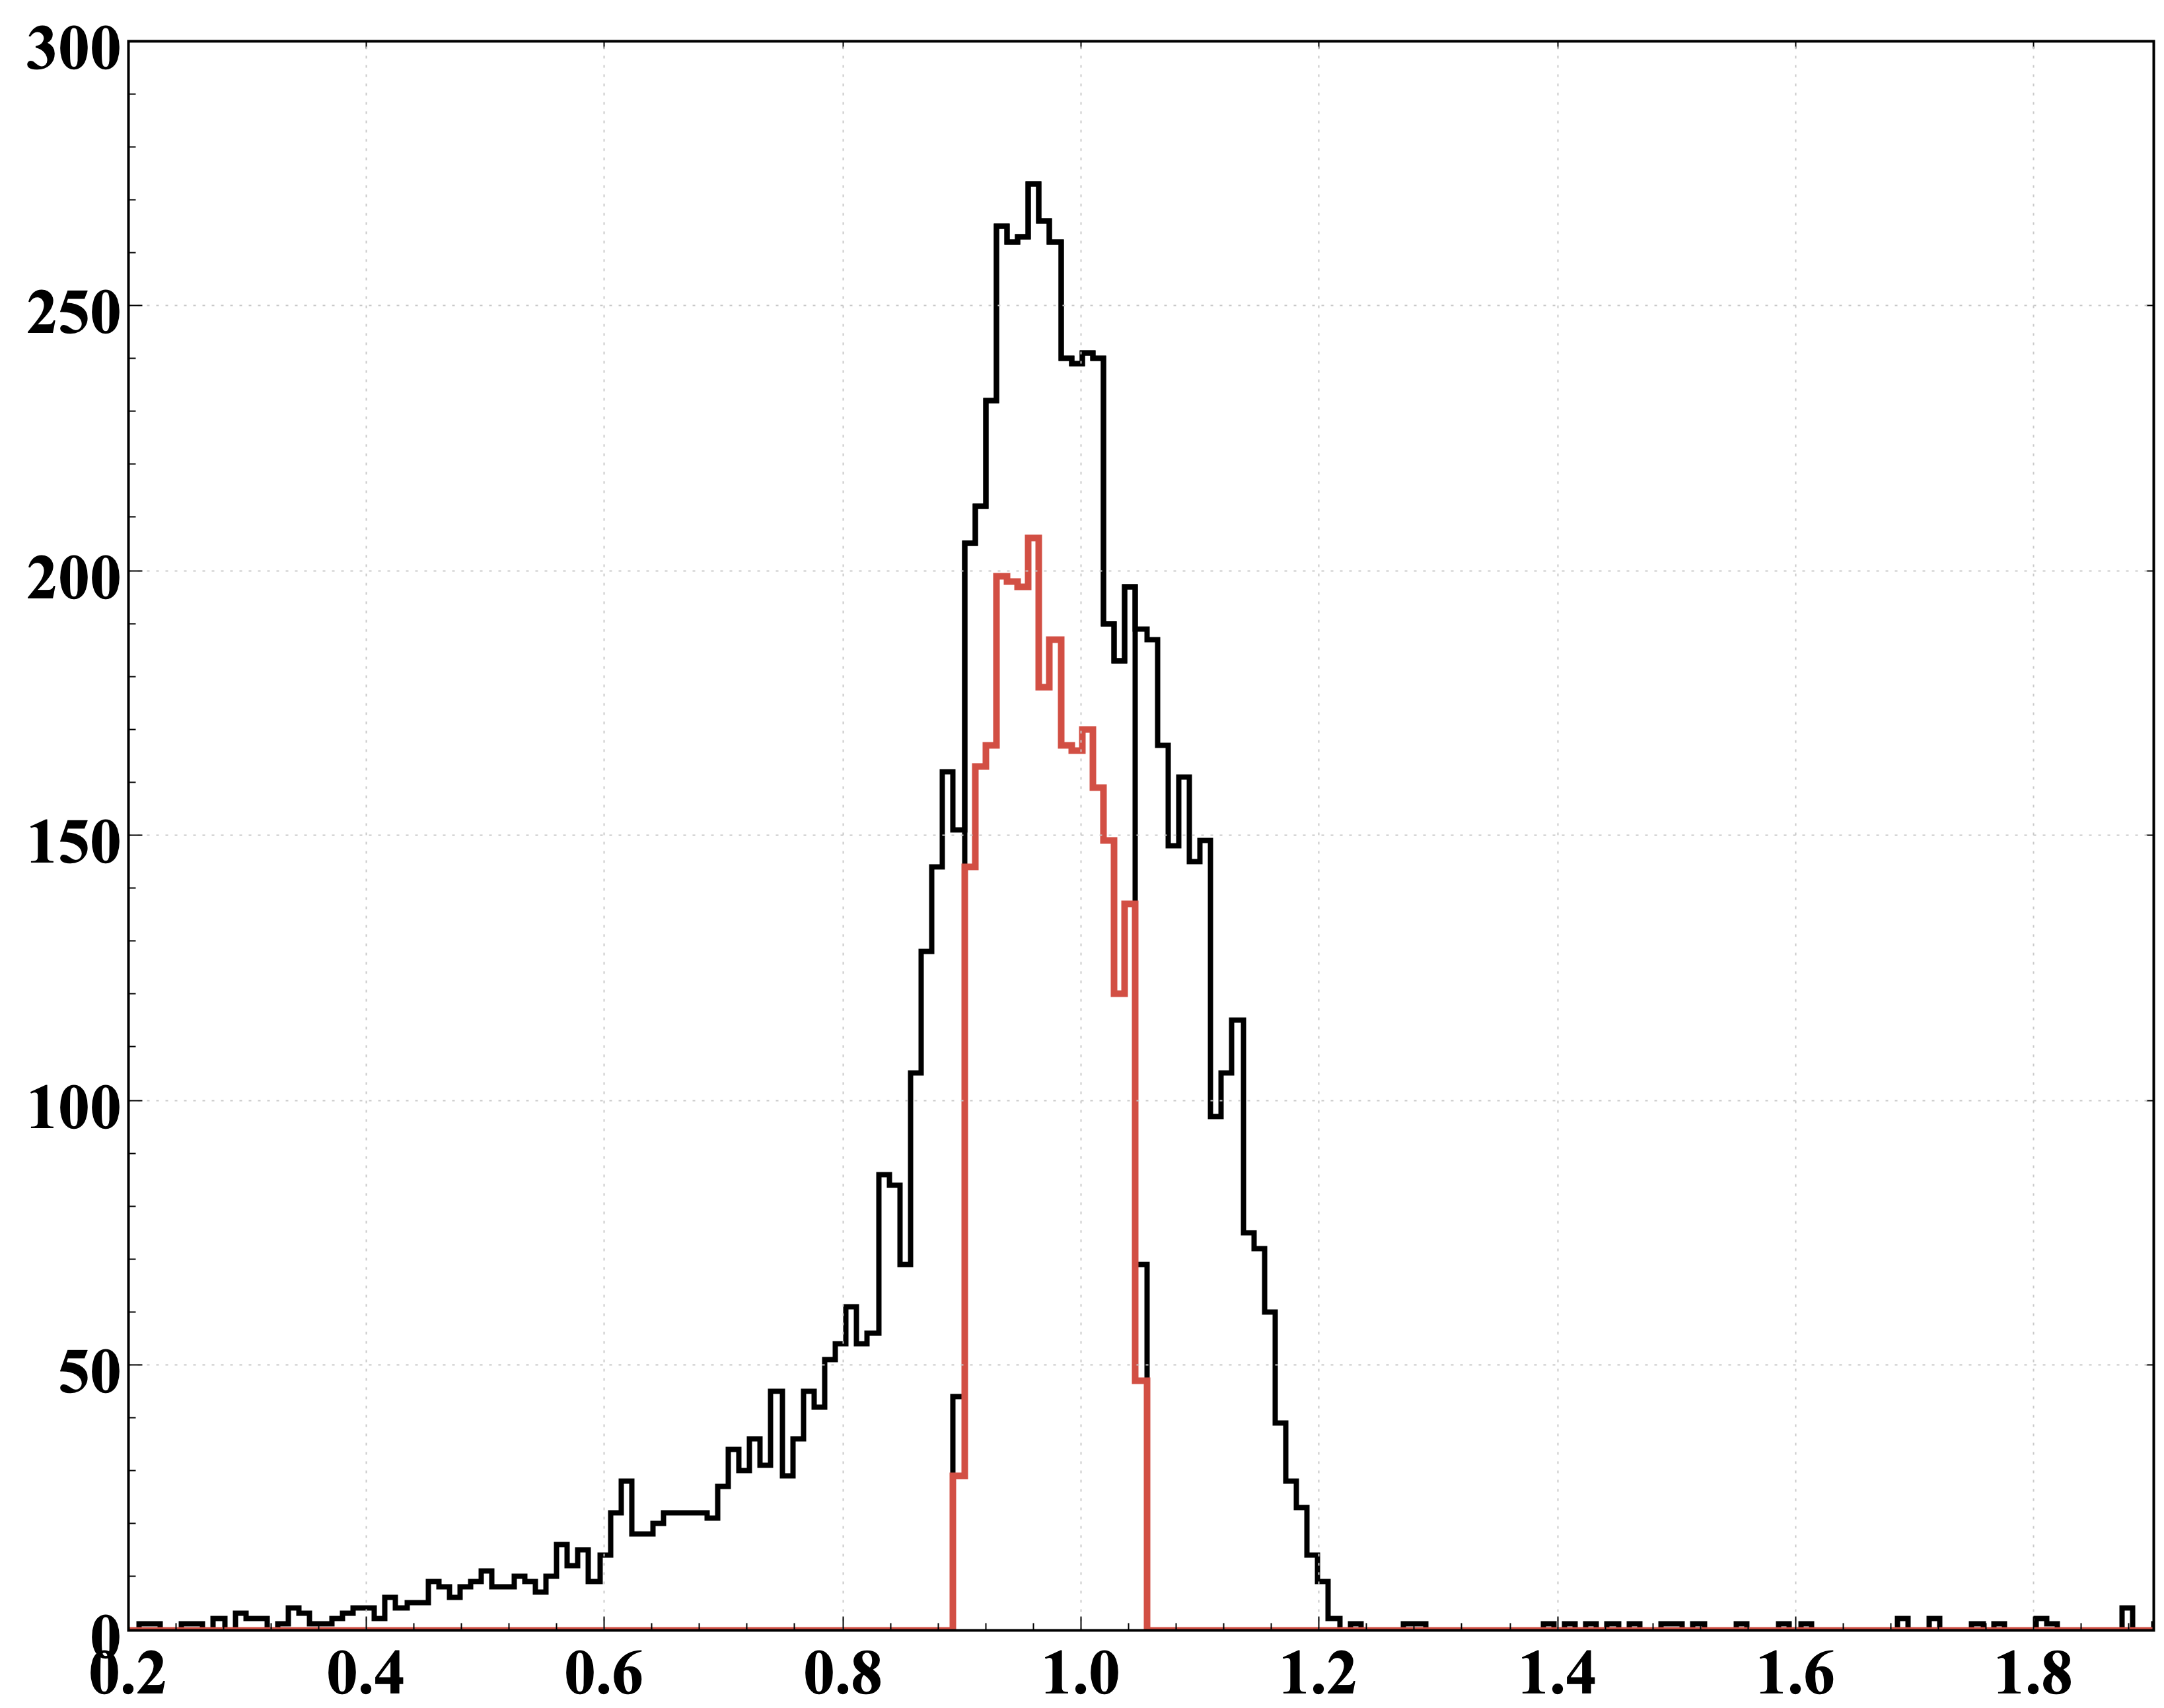
\includegraphics[width=0.98\columnwidth,keepaspectratio]{img/detFiducialCut.png}
	\caption{The missing mass from the reaction $ep \to e'\pi^+X$, where the peak at the neutron mass
          between 0.95 and 1.05~GeV is selected for the efficiency analysis. The positive pion candidates that
          satisfy the cuts are shown in black. The pions associated with an LTCC signal are shown in red.}
	\label{fig:neutronMM}
\end{figure}

\begin{figure}
	\centering
	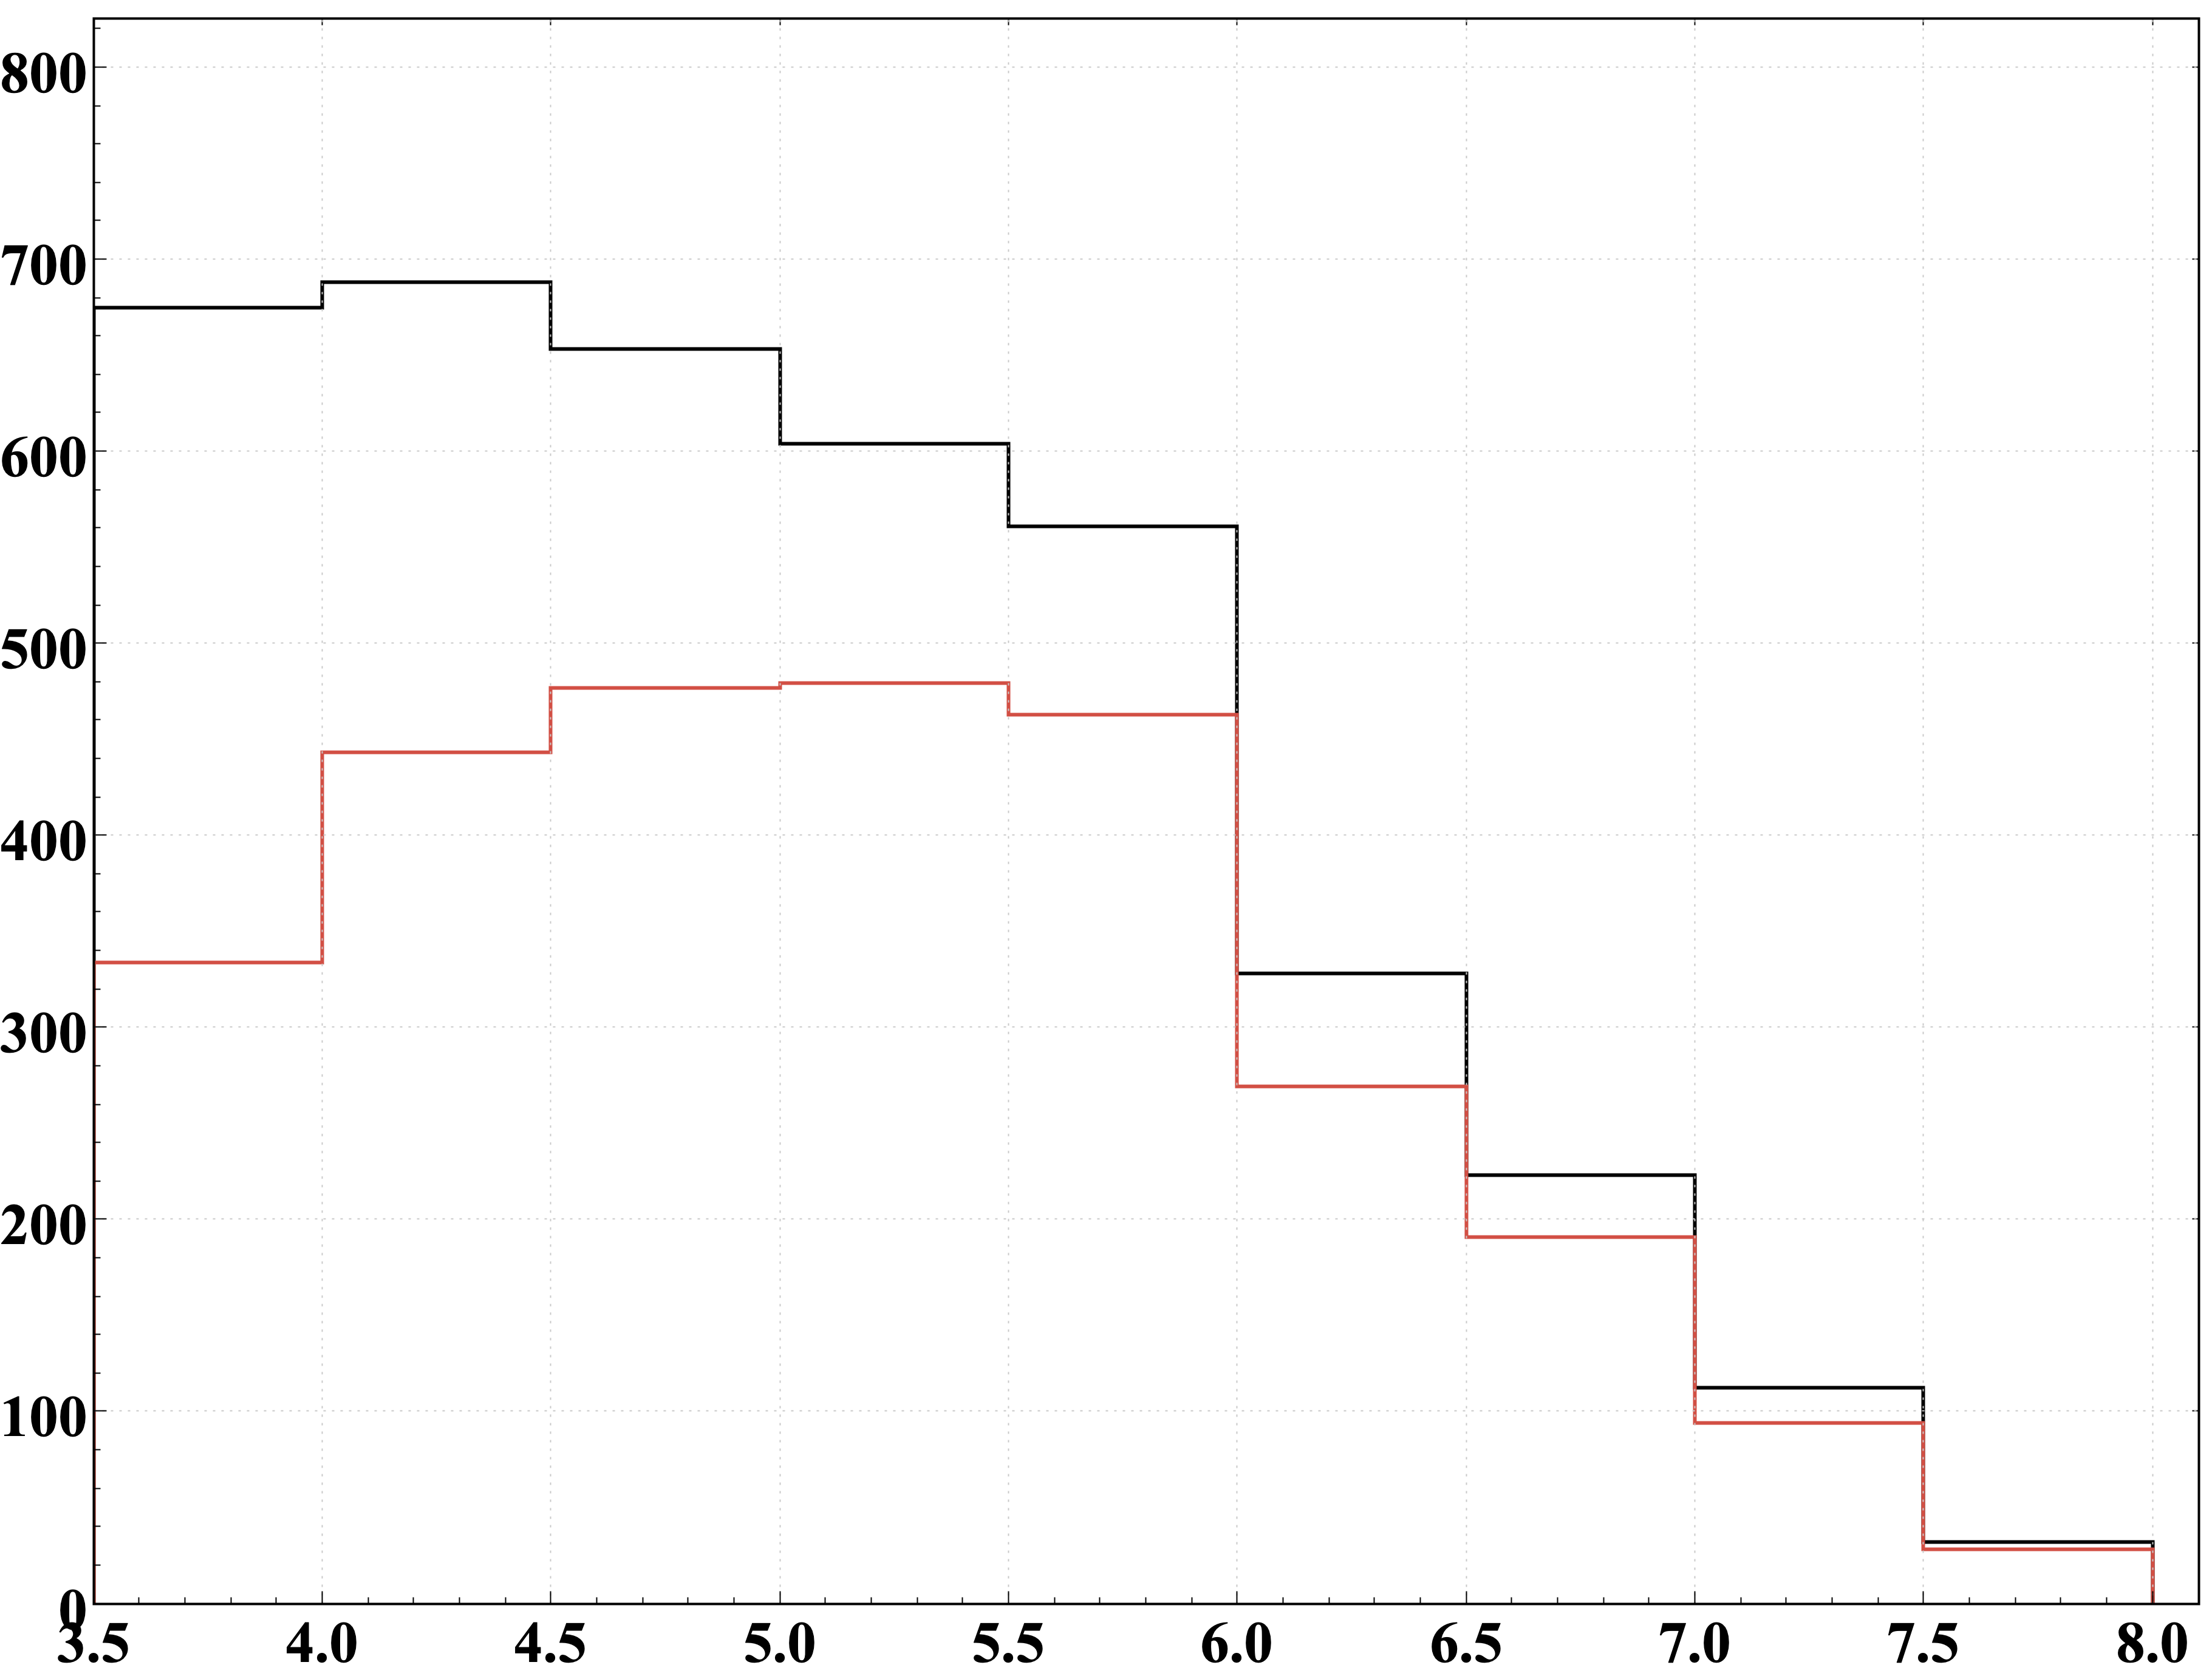
\includegraphics[width=0.98\columnwidth,keepaspectratio]{img/pionMomentum.png}
	\caption{The pion momentum distribution before and after the requirement of an associated LTCC signal. }
	\label{fig:pionMomentum}
\end{figure}

The momentum distribution of the pions is shown in \F{pionMomentum} for the all pions and for the pions
with an associated signal in the LTCC. The ratio defines the LTCC pion detection efficiency as a function of
momentum. Figure~\ref{fig:pionEfficiency} shows the LTCC efficiency for pions normalized to that for electrons
to account for detector inefficiencies unrelated to the LTCC. The LTCC response starts around 50$\%$ near
the expected signal threshold, and rises with momentum as expected. A plateau of 85$\%$ is reached at a
momentum of 5~GeV. This is within range of an expectation of efficiency above 90$\%$. The current LTCC
detector efficiency for pions may be reduced compared to the design expectation by:

\begin{itemize}
   \item the optical alignment of the mirrors, which was a compromise between
	      positive and negative charged tracks instead of optimizing it for negative tracks only;
    \item the  C$_4$F$_{10}$ gas used in the spring 2019 experiment did not go through a purification cycle and
			  may have contained some impurities.
\end{itemize}

\begin{figure}
	\centering
	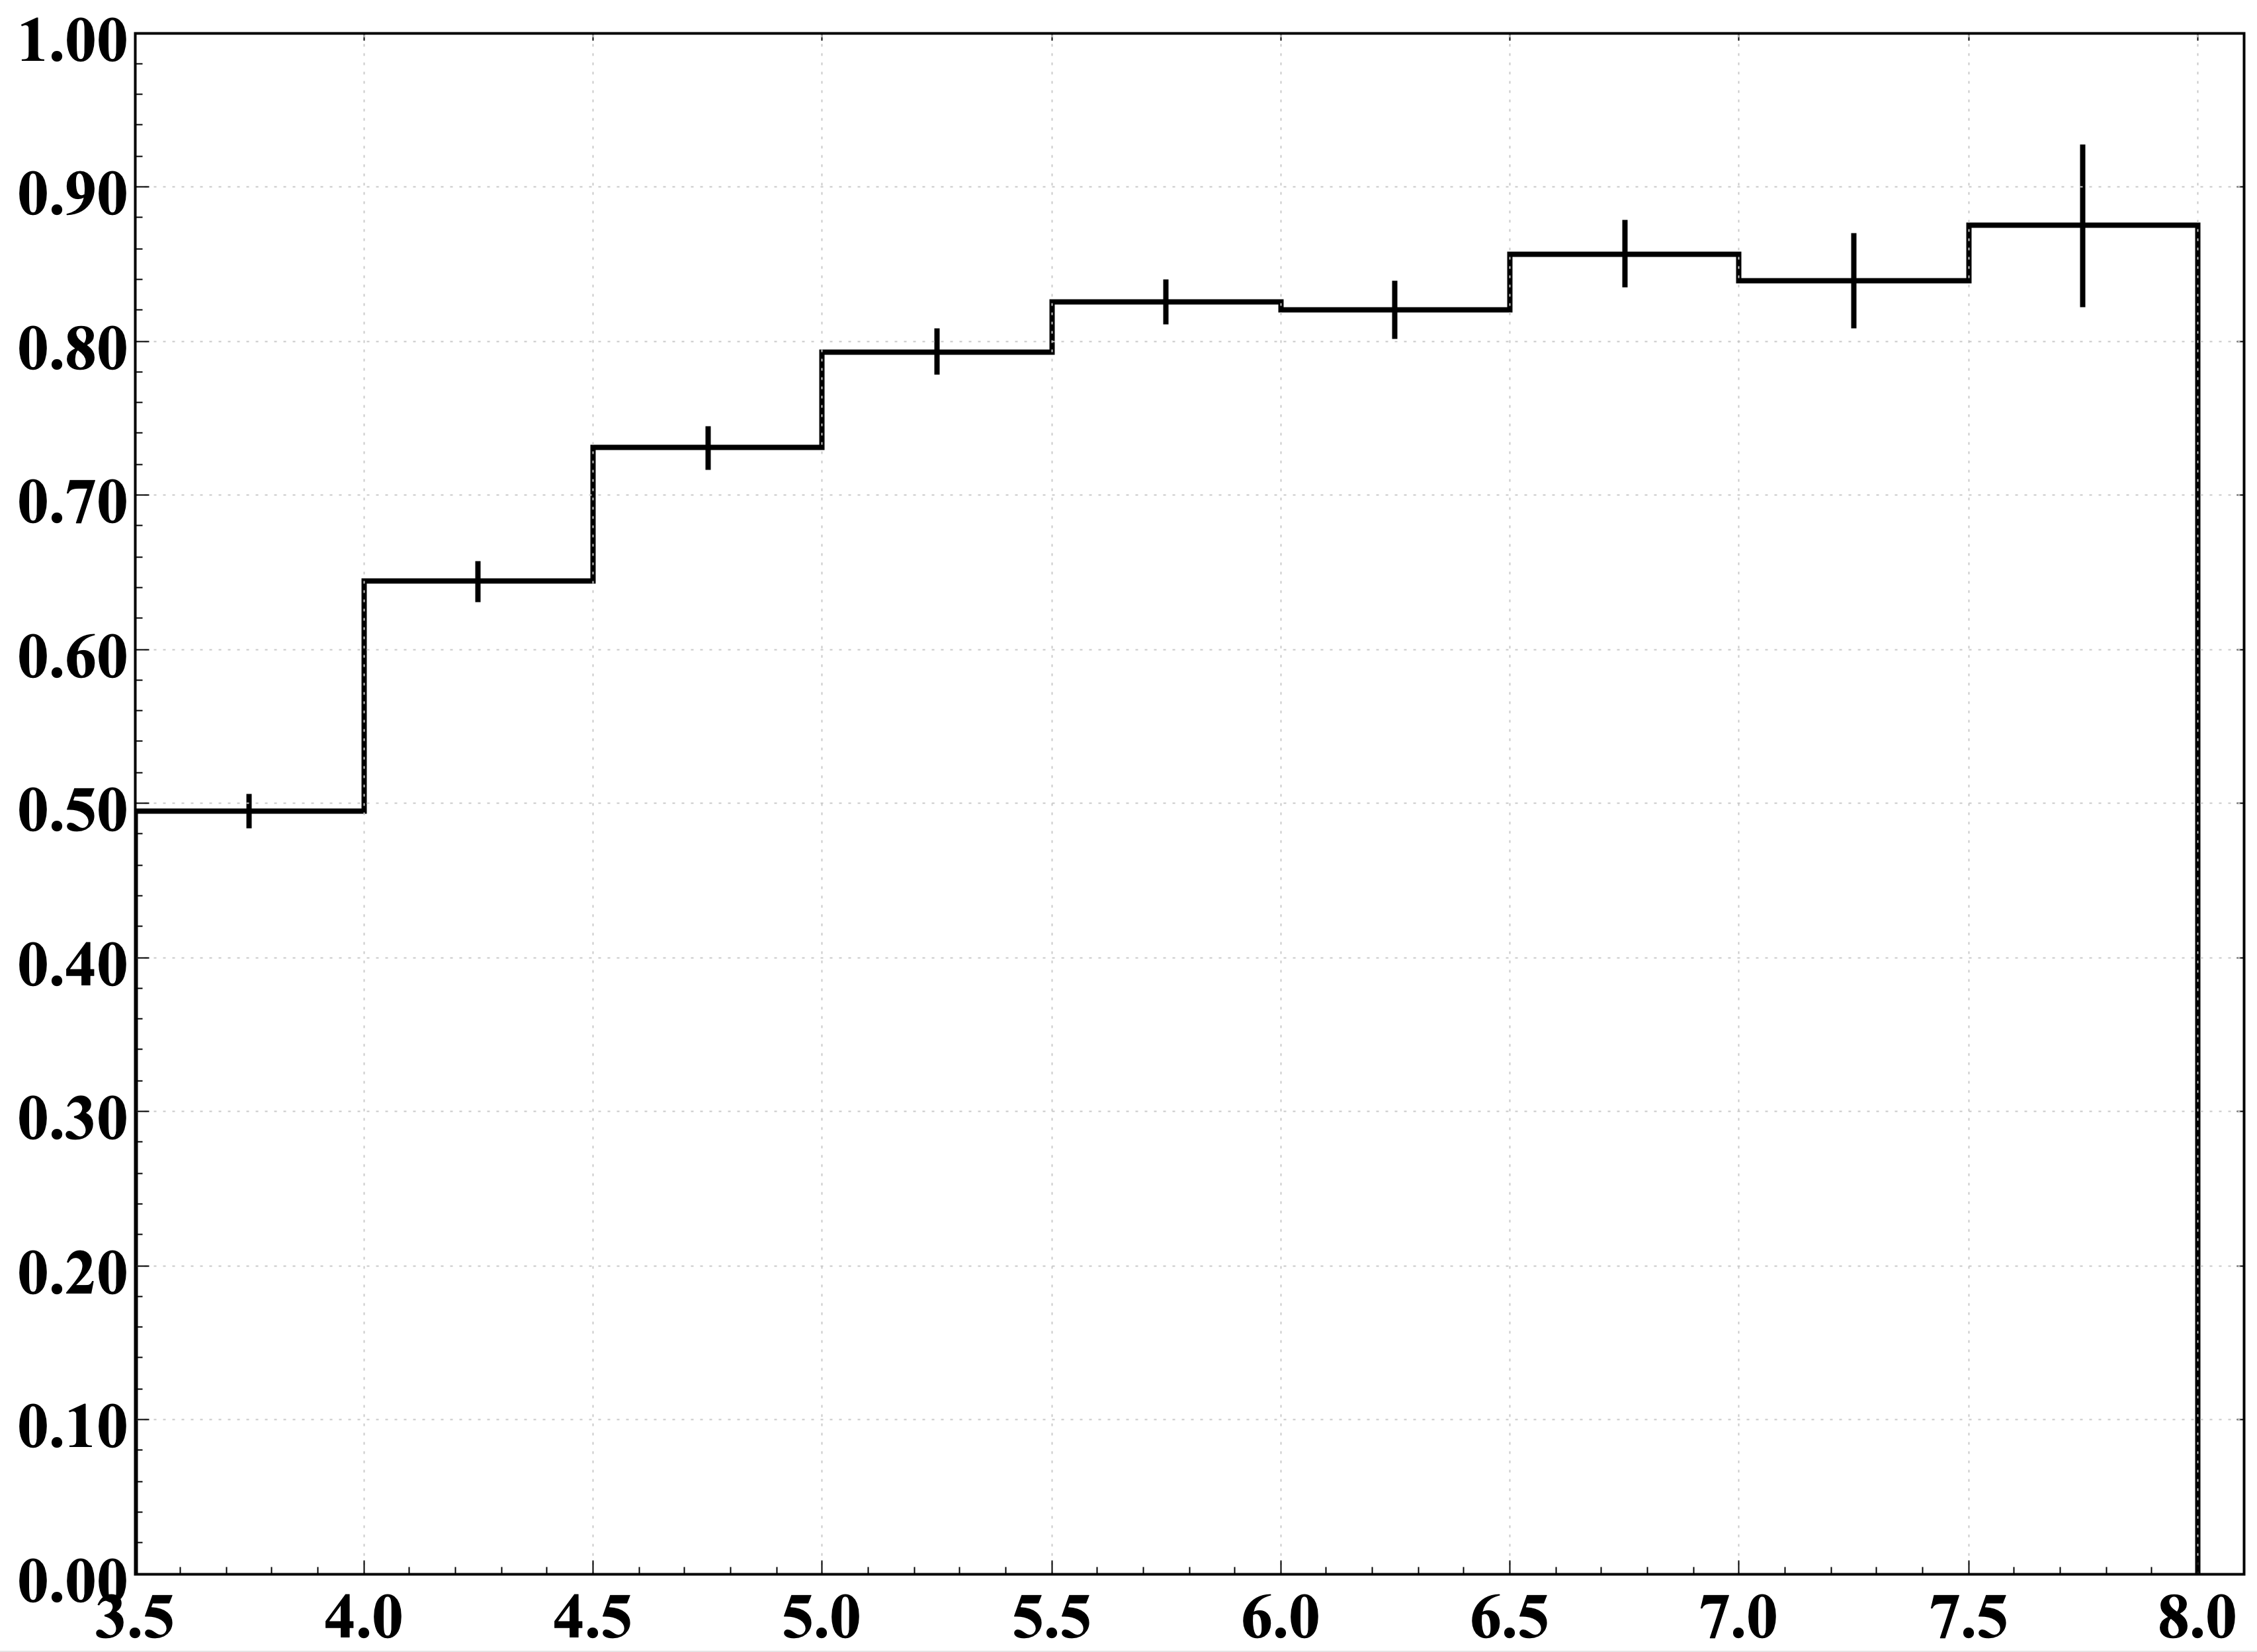
\includegraphics[width=0.98\columnwidth,keepaspectratio]{img/pionEfficiency.png}
	\caption{(placeholder: not normalized to electron yet) The LTCC pion efficiency as a function of momentum.}
	\label{fig:pionEfficiency}
\end{figure}
